\section{Fallbeispiel SAP UI5-Applikation}\label{fallbeispiel}
In diesem Kapitel wird das prototypische Fallbeispiel vorgestellt. Eine kurze Erläuterung des Front- und Backends der Applikation wird in der Beschreibung gegeben. Im Unterkapitel 3.2 werden die genutzten Hilfsmittel in ihrer Funktion und Zugehörigkeit zum Fallbeispiel erklärt. Danach folgt die Implementierung in der, anhand von Screendumps und Applikationscode beschrieben wird, wie das Fallbeispiel nach dem Model-View-Controller Muster umgesetzt worden ist.

\subsection{Beschreibung}
Die prototypische SAP UI5-Applikation ist dazu gedacht, im Rahmen eines SAP SCM-Systems eine Übersicht über die Produkte zu geben. Das Frontend wird im Browser ausgeführt, wohingegen das Backend von einem ABAP AS repräsentiert wird, der zusätzlich noch durch ein SAP NetWeaver Gateway geschützt ist. Nach Auswahl eines Produktes sollen weitere Details angezeigt werden. Auf dieser Detailseite sind Informationen wie Name, Materialnummer, Brutto/Netto Preis und Lagermenge einsehbar. Außerdem können, über zwei Reiter, Charts angezeigt werden. Die erste Chart soll anhand historischer Absatzdaten eine Prognose über zukünftige Absatzzahlen geben. In der zweiten Chart wird eine Bestellvorschau bereitgestellt.

\subsection{Hilfsmittel}
Dieses Kapitel soll aufzeigen, welche Hilfsmittel zur Realisierung des Prototypen verwendet wurden. Zum einen gehört die Entwicklungsumgebung Eclipse dazu. Zum anderen die Chrome-Developer-Tools des Chrome Browser. Im folgenden Unterkapitel werden diese Tools vorgestellt.

\subsubsection{Eclipse}
In der Implementierung des Fallbeispiels ist die quelloffene integrierte Entwicklungsumgebung (IDE) Eclipse zum Einsatz gekommen. Diese IDE wurde von der Eclipse-Foundation entwickelt und ist plattformunabhängig. Geschrieben wurde Eclipse in Java. Die aktuelle Version 4.4 ist am 25. Juni 2014 erschienen und trägt den Namen Luna. Eclipse zeichnet sich durch ein Plugin-System aus, mit welchem eine erhebliche Anzahl an Anwendungsfällen mit der IDE abgedeckt werden können.(vgl. \cite{WikiEclipse2014}) So auch die Entwicklung von SAP UI5-Applikationen. Dafür hat die SAP AG ein spezielles SAP UI5-Plugin bereitgestellt. Entsprechende Plugins müssen nicht umständlich über eine Webseite bezogen und installiert werden. Sie können über die integrierte Plugin Funktion installiert und eingerichtet werden. Eine URL zum Plugin ist vollkommen ausreichend. Für die Entwicklung von SAP UI5-Applikationen wurden folgende Plugins benötigt:
	
\vspace{1em}
\begin{compactitem}
  \item UI Development Toolkit for HTML5
  \item ABAP Development Tools for SAP NetWeaver
  \item (SAP HANA Tools)
\end{compactitem}
\vspace{1em}

Bezogen werden können diese Plugins mittels der erwähnten Pluginfunktion von Eclipse und der URL \url{https://tools.hana.ondemand.com/luna}. Neben dem reinen Code-Editor werden allerdings weitere Tools benötigt, um eine SAP UI5-Applikation zu entwickeln.

\subsubsection{Chrome Developer Tools}
Die SAP UI5-Dokumentation schlägt vor, zum Testen der entwickelten Applikationen, Google Chrome oder Mozilla Firefox anstatt Microsoft Internet Explorer zu verwenden. Das vorliegende Fallbeispiel wurde mit Google Chrome getestet. Google Chrome bietet dazu ein Tool mit dem Namen Developer Tools, welches in jeder Standardinstallation des Browsers enthalten ist. Mit diesem Tool lässt sich beispielsweise das DOM der aktuellen Webseite anzeigen. Weiter kann man JavaScript Breakpoints setzen und so effizient debuggen. Es bietet eine Konsole, um direkte JavaScript Befehle abzusetzen und die Ergebnisse zu analysieren. Um eine Anwendung nicht zwingend auf verschiedenen Endgeräten mit verschiedenen Displaygrößen testen zu müssen, lassen sich jegliche Art von Endgeräten mit den Developer Tools emulieren.(vgl. \cite{DevTools})

%\subsubsection{Neptune Application Designer}

%\subsubsection{Wireframesketcher}
%// Wireframing als Prototyping\\
%// Abbildung Wireframesketcher\\

\subsection{Implementierung}
Es wird die Implementierung des Fallbeispiels beschrieben. Jede Schicht des Model-View-Controller Musters hat dabei ihr eigenes Unterkapitel. Damit werden jeweils die wichtigen Schlüsselpunkte der Applikation offen gelegt. Mehrfach verwendeter Code wird in dem Kapitel bewusst nicht gezeigt, um keine unnötige Komplexität zu erzeugen. Der vollständige Programmcode ist im Anhang zu finden. Abbildung \ref{fig:splitappoverview} zeigt eine schematische Übersicht der SAP UI5-Applikation und ihrer Komponenten.

\vspace{1em}
\begin{figure}[htb]
  \centering
  \includegraphics[width=1\linewidth]{tmp/splitapp_overview}
  \caption[Übersicht der SAP UI5-Applikation]{Übersicht der SAP UI5-Applikation \cite{SAPSplitApp}}
  \label{fig:splitappoverview}
\end{figure}

\subsubsection{Vorbereitungen}
In Eclipse wird ein neues Projekt als SAP UI5-Applikation erstellt. Nach dem Anlegen einer neuen SAP UI5-Applikation ohne anfänglichem View findet man im Projekt Explorer von Eclipse die generierte Verzeichnisstruktur. In dieser Struktur finden sich zu Beginn drei Verzeichnisse. Das \texttt{META-INF} Verzeichnis wird automatisch von Eclipse erstellt und dient lediglich als Informationsspeicher für den Umgang des Projekts im Zusammenspiel mit einigen Java Tools. Daneben existiert das \texttt{WEB-INF} Verzeichnis. In dessen Dateien stehen Anweisungen für das Deployment des Projekts. Zusätzlich sind vorkompilierte Klassendateien und Hilfsbibliotheken in Unterordnern hinterlegt. Außerdem enthält das Projekt auch das \texttt{WebContent} Verzeichnis, welches als Arbeitsverzeichnis für das gesamte Projekt gilt. Dort sind sämtliche statische Dateien, wie z.B. HTML-Dokumente, JavaScript und XML Dateien oder auch andere Ressourcen, wie Bilder und Texte abgelegt.\par Im Arbeitsverzeichnis werden, für die spätere ordentliche Struktur, Verzeichnisse angelegt -- \texttt{i18n}, \texttt{model}, \texttt{util} und \texttt{view}. Im \texttt{i18n} Verzeichnis liegen später die Sprachdateien, um die Applikation lokalisiert auszuliefern. Im \texttt{model} und \texttt{view} Verzeichnis liegen die Views und Modelle der Anwendung. Im \texttt{util} Verzeichnis werden Helferskripte hinterlegt, wie zum Beispiel \texttt{Formatter}- oder \texttt{Grouper}-Skripte. Als Nächstes folgt die Implementierung der Views.

\subsubsection{View}
Die Datei \texttt{index.html} ist der Startpunkt der SAP UI5-Applikation. In dieser Datei wird mittels eines \texttt{title}-Element, direkt unter dem letzten \texttt{meta}-Element, der Seitentitel festgelegt. Innerhalb des folgenden \texttt{script}-Block werden Eigenschaften der SAP UI5-Applikation eingestellt. An dieser Stelle müssen die verwendeten SAP UI5-JavaScript Bibliotheken und die Art und Weise der Datenbindung des Modells hinzugefügt werden. Der Prototyp arbeitet mit der \texttt{complex} Datenbindung.\par In dem leeren \texttt{script}-Block wird letztendlich die Anweisung gesetzt, welche den \textit{Component Container} lädt. Damit wird das Bootstrapping der Applikation in Gang setzt. Die Datei \texttt{index.html} ist in verkürzter Form in Listing \ref{lst:bootstrapping} zu sehen.
	
\vspace{2em}
\begin{lstlisting}[language=HTML5, caption=Bootstrapping der SAP UI5-Applikation, label=lst:bootstrapping]
...
<script
  id="sap-ui-bootstrap"
  src="resources/sap-ui-core.js"
  data-sap-ui-theme="sap_bluecrystal"
  data-sap-ui-libs="sap.m, sap.ui.layout"
  data-sap-ui-preload="" 
  data-sap-ui-xx-bindingSyntax="complex"
  data-sap-ui-resourceroots='{
    "abat.Mockup": "./"
  }' >
</script>

<script>
  new sap.ui.core.ComponentContainer({
    name : "abat.Mockup"
  }).placeAt("content");
</script>
...
\end{lstlisting}
	
\paragraph{Component Container}$\;$ \\
Der im vorangegangenen Absatz erwähnte \textit{Component Container} wird nach den Änderungen an der Datei \texttt{index.html} im Arbeitsverzeichnis als Datei \texttt{Component.js} erstellt. Der \textit{Component Container} ist ein Sammelbehälter für die unterschiedlichen SAP UI5-Komponenten. Er beinhaltet neben der Deklaration und Initialisierung des Modells auch die Root View. Diese Root View ist die unterste Schicht des View Stacks. In ihr werden sämtliche weitere Views platziert. Bei der Initialisierung wird auf die Datei \texttt{App.view.js} verwiesen. Eine nähere Erläuterung der verwendeten Modelle folgt in einem der nächsten Absätze. Als Rückgabewert liefert dieser \textit{Component Container} dann die Root View mit ihren Elementen. Listing \ref{lst:Component.js} zeigt auszugweise die Datei \texttt{Component.js} und die Erstellung des Root View.

\vspace{1em}
\begin{lstlisting}[language=JavaScript, caption=Auszug aus der Datei \texttt{Component.js}, label=lst:Component.js]
var oView = sap.ui.view({
  id : "app",
  viewName : "abat.Mockup.view.App",
  type : "JS",
  viewData : { component : this }
});
return oView;
\end{lstlisting}
	
\paragraph{Root View}$\;$ \\
Die Datei \texttt{App.view.js} repräsentiert die Root View aus dem \textit{Component Container}. Der Rückgabewert ist eine SAP UI5-Komponente, mit dem Namen \texttt{Shell}. Dieser \texttt{Shell} wird ein Titel über das Lokalisierungsmodell zugewiesen. Ausdrücke, die einen String darstellen, können so leicht mit einer lokalen Version des Wertes ersetzt werden. Des Weiteren verlangt die \texttt{Shell} eine \texttt{App} Komponente. Diese Komponente wird am Anfang der Datei \texttt{App.view.js} erzeugt. Es handelt sich bei dem Prototyp um eine \texttt{App} Komponente namens \texttt{SplitApp}. Eine \texttt{SplitApp} besitzt eine Haupt- und Detailseite. Diese werden auch innerhalb der \texttt{App.view.js} erzeugt und der \texttt{SplitApp} Komponente zugewiesen. Allerdings verweisen die Haupt- und Detailseite auch wieder auf eigene Dateien aufgrund des Kapselungsprinzips zum Zwecke der besseren Wartbarkeit. Listing \ref{lst:App.view.js} zeigt den gerade beschriebenen Vorgang.

\vspace{1em}
\begin{lstlisting}[language=JavaScript, caption=Root View der Applikation, label=lst:App.view.js]
...
// create app
this.app = new sap.m.SplitApp();

// load the master page
var master = sap.ui.xmlview("Master", "abat.Mockup.view.Master");
master.getController().nav = this.getController();
this.app.addPage(master, true);

return new sap.m.Shell("Shell", {
  title : "{i18n>ShellTitle}",
  showLogout : false,
  app : this.app
});
...
\end{lstlisting}
	
\paragraph{Hauptseite}$\;$ \\
Die \texttt{Master.view.xml} wird nicht äquivalent der Root View im JavaScript sondern im XML Format erstellt. Sie beinhaltet die Komponenten, die in der \texttt{SplitApp} die Hauptseite darstellt. Realisiert wird das über die Komponente \texttt{Page}. Innerhalb der \texttt{Page} liegen wiederum weitere Komponenten, die das Aussehen der Hauptseite definieren. Durch einen \texttt{customHeader}, inklusive einer \texttt{Bar} und einem \texttt{Image}, wird ein Firmenlogo in die Hauptseite ganz oben eingefügt. Ein \texttt{subHeader}, mit einer \texttt{Bar} und einem \texttt{SearchField}, ist für eine Suchfunktion innerhalb der Liste gesetzt. Eine \texttt{List} implementiert eine vertikale Liste, die mit Komponenten vom Typ \texttt{ObjectListItem} befüllt wird. Das \texttt{ObjectListItem} dient in dem Fall als Formatvorlage für die tatsächlichen Daten, die später aus dem Model bezogen werden. Abgeschlossen wird die Seite mit der \texttt{footer}-Komponente in der eine \texttt{Bar} und ein \texttt{Button} eingelassen sind. Der Button soll eine Gruppierungsfunktion für die Liste möglich machen. Listing \ref{lst:Master.view.xml} enthält die erläuterte Struktur der Hauptseite im XML Format.

\vspace{1em}
\begin{lstlisting}[language=HTML5, caption=Hauptseite der SplitApp, label=lst:Master.view.xml]
<core:View
  controllerName="abat.Mockup.view.Master"
  xmlns="sap.m"
  xmlns:core="sap.ui.core" >
  <Page>
    <customHeader><Bar><contentLeft>
      <Image src="img/logo.png" width="173px" height="30px"></Image>
    </contentLeft></Bar></customHeader>
    <subHeader><Bar><contentLeft>
      <SearchField
        search="handleSearch"
        width="100%" >
      </SearchField>
    </contentLeft></Bar></subHeader>
    <List id="list"
      mode="{device>/listMode}"
      select="handleListSelect"
      items="{/Products}" >
      <ObjectListItem type="{device>/listItemType}"
        press="handleListItemPress"
        title="{MaterialName}"
        number="{Quantity}"
        numberUnit="{i18n&gt;QuantityUnit}"
        numberState="{parts : [ 'Quantity', 'MinimalQuantity' ],
          formatter : 'abat.Mockup.util.Formatter.numberState'}" >
        <attributes>
          <ObjectAttribute text="{MatId}" />
        </attributes>
        <firstStatus><ObjectStatus text="{Status}"
          state="{path: 'Status',
          formatter: 'abat.Mockup.util.Formatter.statusState'}" />
        </firstStatus>
      </ObjectListItem>
    </List>
    <footer>
    <Bar><contentRight><Button icon="sap-icon://group-2"
      press="handleViewSettings" />
    </contentRight></Bar>
    </footer>
  </Page>
</core:View>
\end{lstlisting}

\paragraph{Detailseite}$\;$ \\
Die Detailseite wird zwar in der Root View nicht direkt deklariert, dies erfolgt innerhalb eines Controllers, aber zur Vollständigkeit wird sie erläutert. Vom generellen Aufbau gleicht sie der \texttt{Master.view.xml}. Sie ist auch im XML-Format definiert, enthält aber einige andere Komponenten. Sämtliche Komponenten liegen wieder in einer \texttt{Page}. Begonnen wird mit einem \texttt{ObjectHeader}, dieser setzt den Titel des anzuzeigenden Listeneintrags der Hauptseite. Daneben werden noch weitere Informationen aufgelistet. Unter diesem Kopfteil ist eine \texttt{IconTabBar} platziert. Diese Leiste enthält zwei Einträge, um so später Zugriff auf die beiden Charts zu erhalten. Um auch hier wieder zu kapseln, besitzen die Einträge nur ein Bild und einen Verweis auf ein sogenanntes \texttt{Fragment}. Mit diesem Fragment wird jeweils das Chart definiert, bedeutet die Art des Diagramms und die jeweils dazu spezifischen Einstellungen. Auf ein Listing wird an dieser Stelle verzichtet.

\subsubsection{Modell}
Für die prototypische Implementierung wurde auf ein JSON-Modell gesetzt. So kann die Applikation ohne eine tatsächliche Anbindung an ein SAP-System im Backend getestet werden. Der Aufbau eines JSON-Modells im Vergleich zu einem OData-Modells ist überwiegend gleich bis auf die Tatsache, dass ein OData-Modells noch Metadaten beinhaltet zum OData-Service selbst. Diese Metadaten sind zum Testen der Applikation jedoch nicht vonnöten. Bei einem späteren Produktiveinsatz dieser Applikation kann, durch Veränderung einer Codezeile, das JSON-Modell durch ein OData-Modell ersetzt werden. Natürlich sollte das OData-Modell demzufolge die selbe Struktur besitzen wie das JSON-Modell, da es ansonsten auch zu Komplikationen kommen könnte. Des Weiteren wurde bewusst kein OData-Modell verwendet, da es vom SAP Netweaver Gateway bereitgestellt wird und darauf im Rahmen dieser Arbeit nicht eingegangen werden sollte. Neben dem JSON-Modell, als eigentliche Datenbasis, kommt noch ein Resource-Modell und ein weiteres JSON-Modell zum Einsatz. Das Resource-Modell repräsentiert die Lokalisierung. Dadurch können Strings in den verschiedenen Views dynamisch gesetzt werden. Anhand der Spracheinstellung des dahinter liegenden SAP-Systems wird dann die lokalisierte Variante des String-Wertes verwendet. Die Lokalisierungsdateien liegen in dem \texttt{i18n} Verzeichnis, welches zu Beginn erstellt wurde. Das zweite JSON-Modell stellt ein gerätespezifisches Modell dar. Damit werden Metainformationen über das Gerät gespeichert mit dem die Applikation abgerufen wird. Die dazu nötigen Funktionen werden von der jQuery-Bibliothek bereitgestellt. Die Applikation kann mit diesem Modell ihr visuelles Erscheinungsbild je nach Situation anpassen. In Listing \ref{lst:modelbinding} sind die unterschiedlichen Modelle zu sehen, welche in der Datei \texttt{Component.js} angelegt werden. Jedes Modell wird nach der Erzeugung an dem Root View registriert, damit es im gesamten Applikationskontext zur Verfügung steht.

\vspace{1em}
\begin{lstlisting}[language=JavaScript, caption=Modell an die Root View binden, label=lst:modelbinding]
...
// JSON Modell an die Root View binden
var oModel = new sap.ui.model.json.JSONModel("model/mock.json");
oView.setModel(oModel);

// OData Modell
var oModel = new sap.ui.model.odata.ODataModel(<OData Service URL>);
oView.setModel(oModel);

// I18N(Lokalisierung) Modell
var i18nModel = new sap.ui.model.resource.ResourceModel({
  bundleUrl : "i18n/messageBundle.properties"
});
oView.setModel(i18nModel, "i18n");

// Geraetespezifisches Modell
var deviceModel = new sap.ui.model.json.JSONModel({
  isPhone : jQuery.device.is.phone,
  listMode : (jQuery.device.is.phone) ? "None" : "SingleSelectMaster",
  listItemType : (jQuery.device.is.phone) ? "Active" : "Inactive"
});
deviceModel.setDefaultBindingMode("OneWay");
oView.setModel(deviceModel, "device");
...
\end{lstlisting}

\subsubsection{Controller}
Je View wird mindestens ein Controller vorausgesetzt. Durch den Aufbau der Applikation sind drei Controller nötig. Die Root View benötigt einen allgemeinen Controller, der auch für die beiden anderen Views zuständig ist. Die Haupt- und Detailseite haben jeweils ihren eigenen Controller, der nur auf Benutzeraktionen des jeweiligen View reagiert. Einerseits um Daten aus dem Modell zu beziehen, andererseits um Navigationsaktionen an den Root Controller weiterzugeben.

\paragraph{Controller Root View}$\;$ \\
Der Root-Controller implementiert zwei Funktionen zur Navigation. Mit diesen beiden Funktionen lässt sich beispielsweise von der Detailseite zurück auf die Hauptseite navigieren und andersherum. Des Weiteren veranlasst die \texttt{to} Funktion die Applikation dazu direkt beim ersten Aufruf die Hauptseite zu laden, damit kein leerer Bildschirm angezeigt wird. Dieser Mechanismus ist in Listing \ref{lst:navigation} gezeigt.

\vspace{1em}
\begin{lstlisting}[language=JavaScript, caption=Navigationsmechanismus, label=lst:navigation]
...
to : function (pageId, context) {
  var app = this.getView().app;

  // load page on demand
  var master = ("Master" === pageId);
  if (app.getPage(pageId, master) === null) {
    var page = sap.ui.view({
      id : pageId,
      viewName : "abat.Mockup.view." + pageId,
      type : "XML"
    });
	page.getController().nav = this;
	app.addPage(page, master);
	jQuery.sap.log.info("app controller > loaded page: " + pageId);
  }

  // show the page
  app.to(pageId);

  // set data context on the page
  if (context) {
    var page = app.getPage(pageId);
    page.setBindingContext(context);
  }
},
...
\end{lstlisting}

\paragraph{Controller Hauptseite}$\;$ \\
Im Controller der Hauptseite sind sämtliche \textit{Handler} untergebracht, die zu Komponenten der Seite gehören. Ein relativ einfach zu implementierender, aber trotzdem absolut wichtiger \textit{Handler}, ist \texttt{handleListItemPress}. Dieser \textit{Handler} wird ausgeführt, sobald in der Liste der Hauptseite ein Eintrag gedrückt bzw. ausgewählt wird. Bevor direkt die Detailseite aufgerufen wird, holt sich die Funktion noch den aktuellen Datenkontext des Eintrags. Diesen Kontext gibt er an die Navigationsfunktion aus dem Root-Controller weiter. Dadurch muss der Controller der Detailseite nicht erst die Daten beschaffen, sondern die Detail View kann die Informationen direkt aus dem übergebenen Kontext entnehmen und darstellen. Das reduziert den Datentraffic zwischen Controllern und Modell und dementsprechend auch die Verbindungen zum Backend-System. Ein weiterer \textit{Handler} ist implementiert, um die Suchfunktion der Liste zu realisieren. Sobald eine Suche gestartet wird, reagiert diese Funktion darauf und filtert die Liste anhand des eingegebenen Suchwortes. Dazu stellt das SAP UI5-Framework ein Filter Objekt zur Verfügung. Diesem Filter-Objekt übergibt man die Eigenschaft aus dem Modell nach der gefiltert werden soll. Der zweite Parameter ist eine Konstante aus dem SAP UI5-Framework, die den entsprechenden Filter-Operator angibt. In diesem Fall wird geprüft, ob die Eigenschaft den Suchbegriff enthält. Der letzte Parameter ist das Suchwort selbst. In Listing \ref{lst:navsearch} sind die beschriebenen \textit{Handler} Funktionen abgebildet.

\vspace{1em}
\begin{lstlisting}[language=JavaScript, caption=Navigation und Suchfunktion der Hauptseite, label=lst:navsearch]
...  
// Handler Listenelemnte
handleListItemPress : function (evt) {
  var context = evt.getSource().getBindingContext();
  this.nav.to("Detail", context);
},
handleListSelect : function (evt) {
  var context = evt.getParameter("listItem").getBindingContext();
  this.nav.to("Detail", context);
},
  
// Handler Suchfunktion
handleSearch : function (evt) {		
  // create model filter
  var filters = [];
  var query = evt.getParameter("query");
  if (query && query.length > 0) {
    var filter = new sap.ui.model.Filter("MaterialName",
      sap.ui.model.FilterOperator.Contains, query);
    filters.push(filter);
  }	
  // update list binding
  var list = this.getView().byId("list");
  var binding = list.getBinding("items");
  binding.filter(filters);
},
...
\end{lstlisting}

Da die Liste auch eine Möglichkeit zur Gruppierung bieten soll, wurde ein weiterer \textit{Handler} implementiert. Dieser \textit{Handler} reagiert, sobald auf der Hauptseite der Button unter der Liste gedrückt wird. Die Funktion erzeugt daraufhin ein Dialogfenster und stellt direkt dazu die Eigenschaften ein. So kann anhand des Bruttopreises und des Status' gruppiert werden. Außerdem benötigt der Dialog noch eine Funktion, welche die Benutzereingabe entsprechend verarbeitet je nachdem für welche Gruppierung sich der Anwender entschieden hat. Um diese Entscheidung korrekt umzusetzen, wurde ein Hilfsskript implementiert, welches im \texttt{util} Verzeichnis als Datei \texttt{Grouper.js} abgelegt ist. Dieses Hilfsskript liefert, je nach Gruppierungskriterium, die entsprechenden Werte aus dem Kontext. Da im Dialog auch eine Auswahl bezüglich der Sortierung vorhanden ist, wird auch dies mit in die Gruppierung einbezogen. SAP UI5 stellt auch dafür eine fertige Funktion zur Verfügung. Listing \ref{lst:listgrouping} zeigt die implementierte Funktion aus dem Controller.

\vspace{1em}
\begin{lstlisting}[language=JavaScript, caption=Handler der Listengruppierung, label=lst:listgrouping]
...
// Handler Listengruppierung
handleViewSettings : function (evt) {
  var that = this;
  if (!this._lineItemViewDialog) {
    // create dialog
    this._lineItemViewDialog = new sap.m.ViewSettingsDialog({
      groupItems : [
        new sap.m.ViewSettingsItem({
          text : "Price",
          key : "GrossAmount"
        }),
        new sap.m.ViewSettingsItem({
          text : "Status",
          key : "Status"
        })],
      confirm : function (evt) {
        var aSorters = [];
        var mParams = evt.getParameters();
        if (mParams.groupItem) {
          var sPath = mParams.groupItem.getKey();
          var bDescending = mParams.groupDescending;
       	  var vGroup = abat.Mockup.util.Grouper[sPath];
       	  aSorters.push(new sap.ui.model.Sorter(
       	    sPath, bDescending, vGroup));
        }
        var oBinding = that.getView().byId("list")
          .getBinding("items");
        oBinding.sort(aSorters);
      }
    });
  }
  this._lineItemViewDialog.open();
}
...
\end{lstlisting}

\paragraph{Controller Detailseite}$\;$ \\
Der Controller der Detailseite hat als wichtigste Aufgabe die Charts zu konfigurieren, die unter der Kopfzeile angezeigt werden. Im SAP UI5-Framework ist eine eigene Klasse für die Chartvisualisierung enthalten, welche einen großen Umfang an verschiedenen Chartstyles besitzt. Im Prototyp wurden zunächst nur Bar- und Line-Charts verwendet. Ein Chart benötigt eine Datenbasis auf die es sich stützt. Diese Datenbasis bildet im Prototyp das globale Modell. Da die Detailseite bei einem Aufruf aus der Hauptseite automatisch den Datenkontext des gewählten Listeneintrags mitbekommt, kann in der Datenbasis des Charts, dem \texttt{FlattenedDataset}, einfach auf einen Pfad, innerhalb des JSON-Modell, Bezug genommen werden. Daneben werden noch die Achsen entsprechend der Verwendung eingestellt und benannt. Anhand der, in dem View festgelegten, ID wird das Chartobjekt dann referenziert. Es wird ein Titel festgelegt, welcher ebenfalls über eine lokalisierte Variante verfügt. Zuletzt wird das erstellte \texttt{FlattenedDataset} an das Chart gebunden.

\vspace{1em}
\begin{lstlisting}[language=JavaScript, caption=Chart Konfigurierung, label=lst:chartconfig]
...
handleNavButtonPress : function (evt) {
  this.nav.back("Master");
},
...
	
configForecastChart : function () {
  var oDatasetForecast = new sap.viz.ui5.data.FlattenedDataset({
  dimensions : [{
    axis : 1,
    name : 'Month',
    value : "{Month}"
  }],
  measures : [{
    name : 'Menge1',
    value : '{Menge1}'
    },{
    name : 'Menge2',
    value : '{Menge2}'
  }],		
  // data comes from model
  data : {
    path : "ForecastData"
  }
  });

  oLineChart = this.getView().byId("lineChart");
  oLineChart.setTitle(new sap.viz.ui5.types.Title(
        {visible:true, text:"{i18n>ForecastChartTitle}"}));
  oLineChart.setDataset(oDatasetForecast);
},
\end{lstlisting}

\subsubsection{Deployment}
Sofern das Backend-System entsprechend vorbereitet ist - alle SAP UI5-Addons und Patches eingespielt und aktiviert - verläuft das Deployment der Applikation relativ schnell und einfach. Eclipse bietet dazu eine eigene Funktion an, mit der sich ein angelegtes Projekt auf verschiedenste Plattformen deployen lässt. In Abbildung \ref{fig:eclipseshare} ist der entsprechende Menüeintrag zu sehen, welcher über einen Rechtsklick auf das Projekt zu erreichen ist.

\vspace{1em}
\begin{figure}[htb]
  \centering
  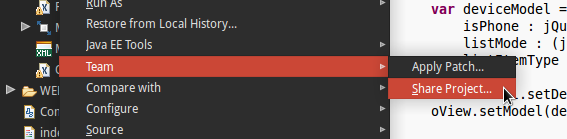
\includegraphics[width=0.8\linewidth]{abb/eclipse_share_project}
  \caption[Eclipse Menüeintrag zum deployen des Projekts]{Eclipse Menüeintrag zum deployen des Projekts}
  \label{fig:eclipseshare}
\end{figure}

Durch die SAP UI5-Plugins steht unter dieser Funktion auch ein SAP-System als Zielplattform zur Verfügung. Nach der Auswahl des SAPUI5-ABAP-Repository erscheint ein weiteres Fenster, in welchem die Verbindungsdaten des SAP-Systems eingetragen wurden. Nach erfolgreichem Verbindungstest werden noch einige zusätzliche Informationen zu dem SAP-System angezeigt. Im nächsten Schritt verlangt Eclipse die Eingabe der SAP Logindaten.

\vspace{1em}
\begin{figure}[htb]
  \centering
  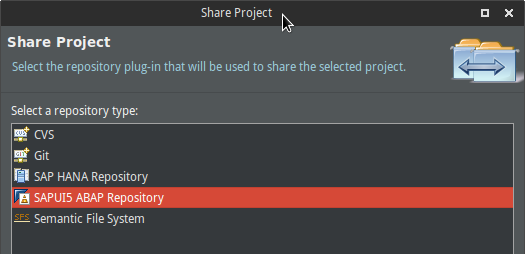
\includegraphics[width=0.8\linewidth]{abb/eclipse_share_project_window}
  \caption[Remote Repository Auswahl in Eclipse]{Remote Repository Auswahl in Eclipse}
  \label{fig:eclipsesharewindow}
\end{figure}

Ist Eclipse vollständig mit dem SAP-System verbunden, kann das Projekt entweder in eine schon existierende BSP-Applikation deployed werden oder es kann eine komplett neue BSP-Applikation über Eclipse auf dem SAP-System angelegt werden. Letztere Möglichkeit wurde mit dem Prototyp verwendet. Name, Beschreibung und ein Paket sind dazu nötig. Der Name und das Paket müssen sich im \textit{Z*}-Namensraum befinden. Die Beschreibung kann frei gewählt werden. Einen Schritt weiter erfolgt die Auswahl eines Transportauftrags, sofern im Entwicklungssystem ein Transportauftrag vorhanden ist. Daraufhin lässt sich über einen erneuten Rechtsklick auf das Projekt selbiges an das zuvor eingestellte SAP-System schicken. Auf dem SAP-System selbst wird danach die BSP-Applikation angelegt und der entsprechende Service in der Transaktion \texttt{SICF} erstellt und aktiviert. Ab diesem Zeitpunkt ist der Prototyp unter der entsprechenden URL im Browser aufrufbar.\par Ruft man nun die URL des Prototypen im Browser auf baut sich die Applikation auf und erwartet die Eingabe des Anwenders. Nach einem Klick auf einen Listeneintrag am linken Rand der Anwendung erscheint im rechten Bereich der Seite der Detailbereich mit nähern Informationen zum gewählten Eintrag. Außerdem ist im unteren Teil des rechten Bereichs eine Chart angezeigt. Abbildung \ref{fig:prototypsplitapp} zeigt den Prototypen.

\vspace{1em}
\begin{figure}[htb]
  \centering
  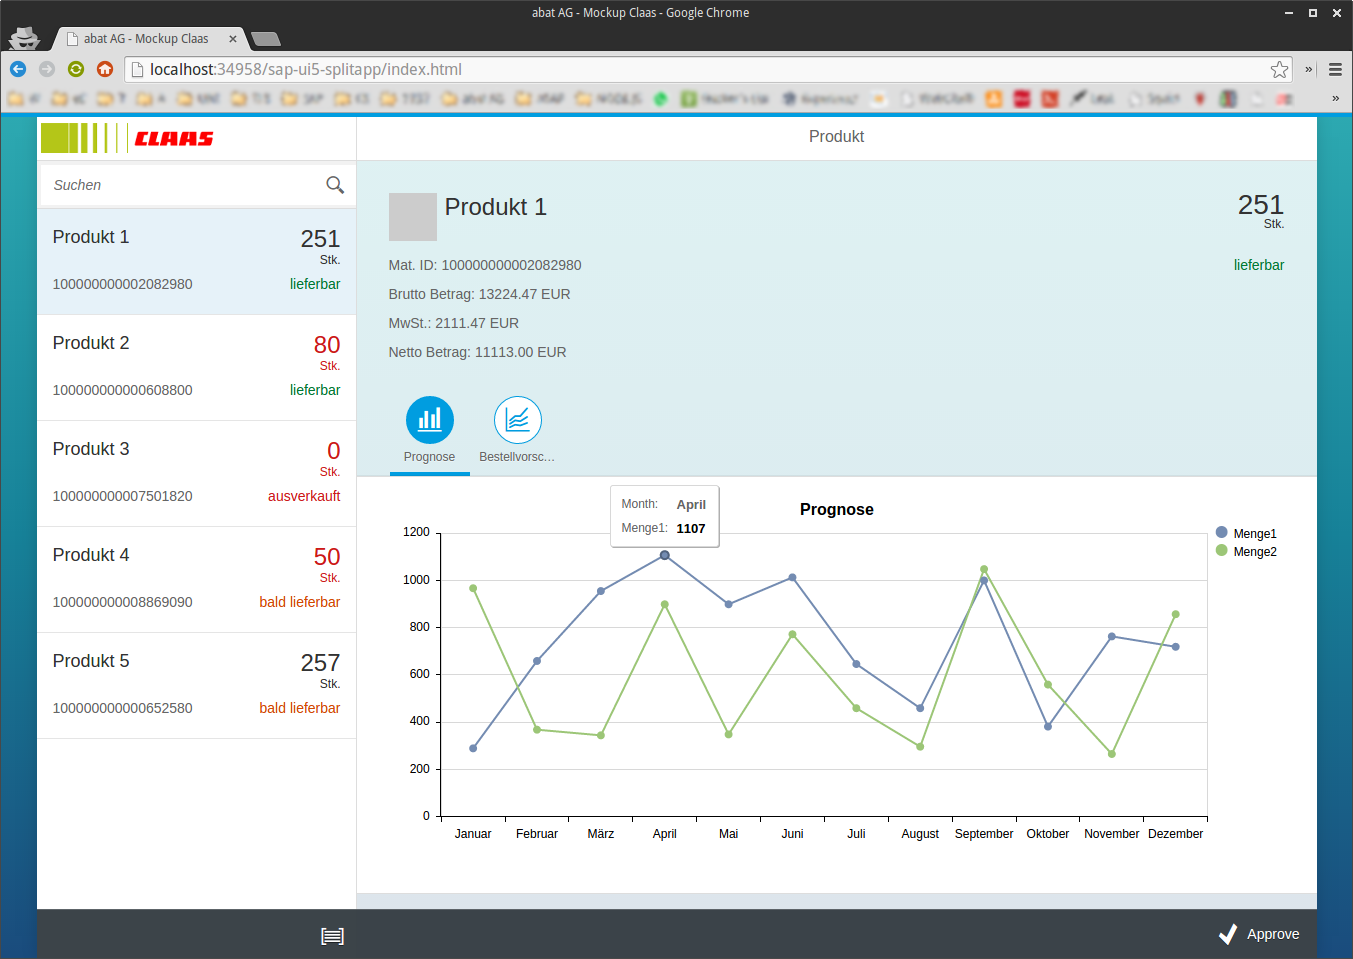
\includegraphics[width=1\linewidth]{abb/sapui5_final_splitapp}
  \caption[Prototyp SAP UI5-Applikation]{Prototyp SAP UI5-Applikation}
  \label{fig:prototypsplitapp}
\end{figure}